\documentclass{beamer}
\usetheme{Boadilla}
\usepackage{hyperref}
\usepackage{tikz}
\usetikzlibrary{shapes,positioning}
\usepackage{graphicx}
\usepackage{fontawesome}
\usepackage{fancyvrb}
\usepackage{adjustbox}
\usepackage{multicol}
\usepackage{subfig}
\usepackage{xcolor}
\usepackage{optparams}
\usepackage{xstring}
\usepackage[
    backend=biber, 
    natbib=true,
    style=numeric,
    sorting=none,
    style=verbose-ibid,
]{biblatex}
\addbibresource{citations.bib}
\usepackage{pgfpages}
\definecolor{ao(english)}{rgb}{0.0, 0.5, 0.0}
\definecolor{burgundy}{rgb}{0.5, 0.0, 0.13}
\setbeameroption{show notes}
\setbeameroption{show notes on second screen=right}
%\setbeameroption{hide notes}

\def\footshortciteintern[#1][#2]#3{%
\ifx#1\empty 
% Nur Autor
\footnote{\citeauthor{#3}, \citeyear{#3}.}
\else
\ifx#2\empty
% Autor und Seite
\footnote{\citeauthor{#3}, \citeyear{#3}, #1.}
\else
% Autor, Seite und vgl.
\expandafter  
\footnote{\citeauthor{#3}, \citetitle{#3}, \citeyear{#3}, \citeurl{#3}.}
\fi
\fi
}
\newcommand*\footshortcite{%
\optparams{\footshortciteintern}{[\empty][\empty]}
}
\newcommand*\footmediumcite{%
\optparams{\footshortciteintern}{[][]}
}


\title{Structured Sparsity}
\subtitle{Final project presentation}
\author{Sevag Hanssian}
\date{April 22, 2021}
\institute{MUMT 622, Winter 2021}
\setbeamertemplate{navigation symbols}{}

\begin{document}

\begin{frame}
\maketitle
\end{frame}

\begin{frame}
\end{frame}

\begin{frame}
	\frametitle{Structured sparsity}
	Group-LASSO:\footfullcite{sparsitykowalski} solve the problem of finding signifiance maps (i.e. locations of significant coefficients) in the transform domain
	\begin{figure}
		\vspace{-0.25em}
		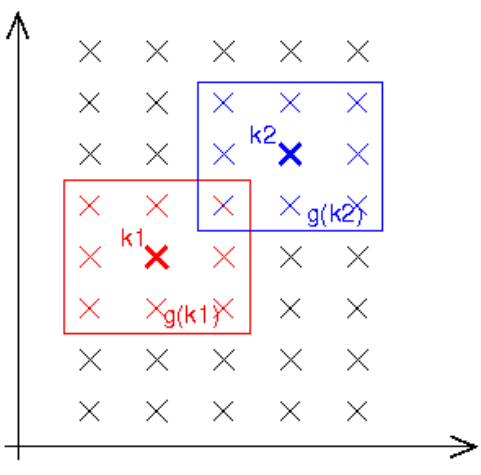
\includegraphics[width=3.5cm]{./grouplasso.png}
		\caption{Group-LASSO regression on two overlapping groups}
		\vspace{-1em}
	\end{figure}
	Sparsity is the property of concentrating most of the energy of a signal $x$ in few coefficients of transform $w$\footshortcite{pastor2015mathematics}
\end{frame}

\begin{frame}
	\frametitle{Structured sparsity}
	WMDCT\footfullcite{wmdct} + Group-LASSO -- ``audioshrink''\footnote{\url{https://homepage.univie.ac.at/monika.doerfler/StrucAudio.html}, \url{https://ltfat.github.io/doc/demos/demo_audioshrink.html}}
	\begin{figure}[ht]
		\vspace{-0.5em}
		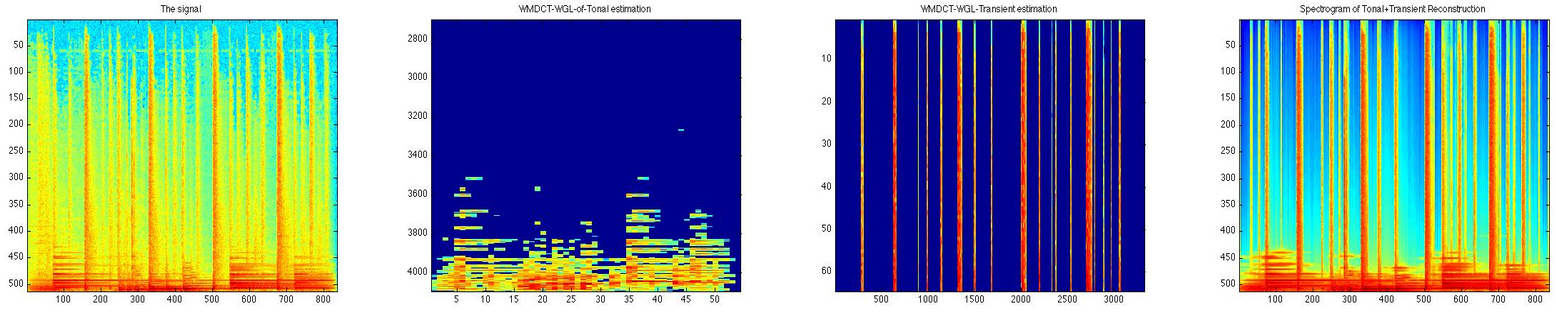
\includegraphics[width=11cm]{./wmdctjazz.png}
		\caption{Audioshrink for tonal/transient separation in jazz music}
		\vspace{-0.5em}
	\end{figure}
	Use 2 WMDCT transforms (wide + narrow window) + Group-LASSO to shrink input signal into significant coefficients in ``time'' and ``frequency'' groups
\end{frame}

\end{document}
